\chapter{Экспериментальный раздел}
\label{cha:research}


\section{Технические характеристики}
Тестирование выполнялось на устройстве \cite{lenovo} со следующими техническими характеристиками:
\begin{itemize}
	\item Операционная система Ubuntu 20.04.03 LTS;
	\item Память 16 GiB (4,5 GiB выделено для нужд графического ядра)
	\item Процессор AMD® Ryzen 5 5500u --- 12 потоков
    \item Видеопроцессор AMD® Radeon RX Vega 7 --- 448 потоков
\end{itemize}

\section{Время выполнения алгоритмов}

Для замеров времени использовалась стандартного класса языка С++ \verb|std::chrono::high_resolution_clock|. Данный класс предоставляет интерфейс замеров времени с максимальной возможной точностью.

\subsection{Анализ времени работы этапов построения изображения}

Был произведен замер времени генерации изображения, разбитый на логические этапы. При тестировании на сцене (представлена на рисунке \ref{fig:scene_exp}) были видимы 7 моделей, разрешение генерируемого изображения 1848x1016 пикселей, 20 семплов методов размытия и размер участка изображения 40x40 пикселей. В данной сцене камера следует за движущемся автомобилем. Результаты замеров приведены в таблице \ref{tbl:time}. 


\begin{figure}[h]
    \centering
    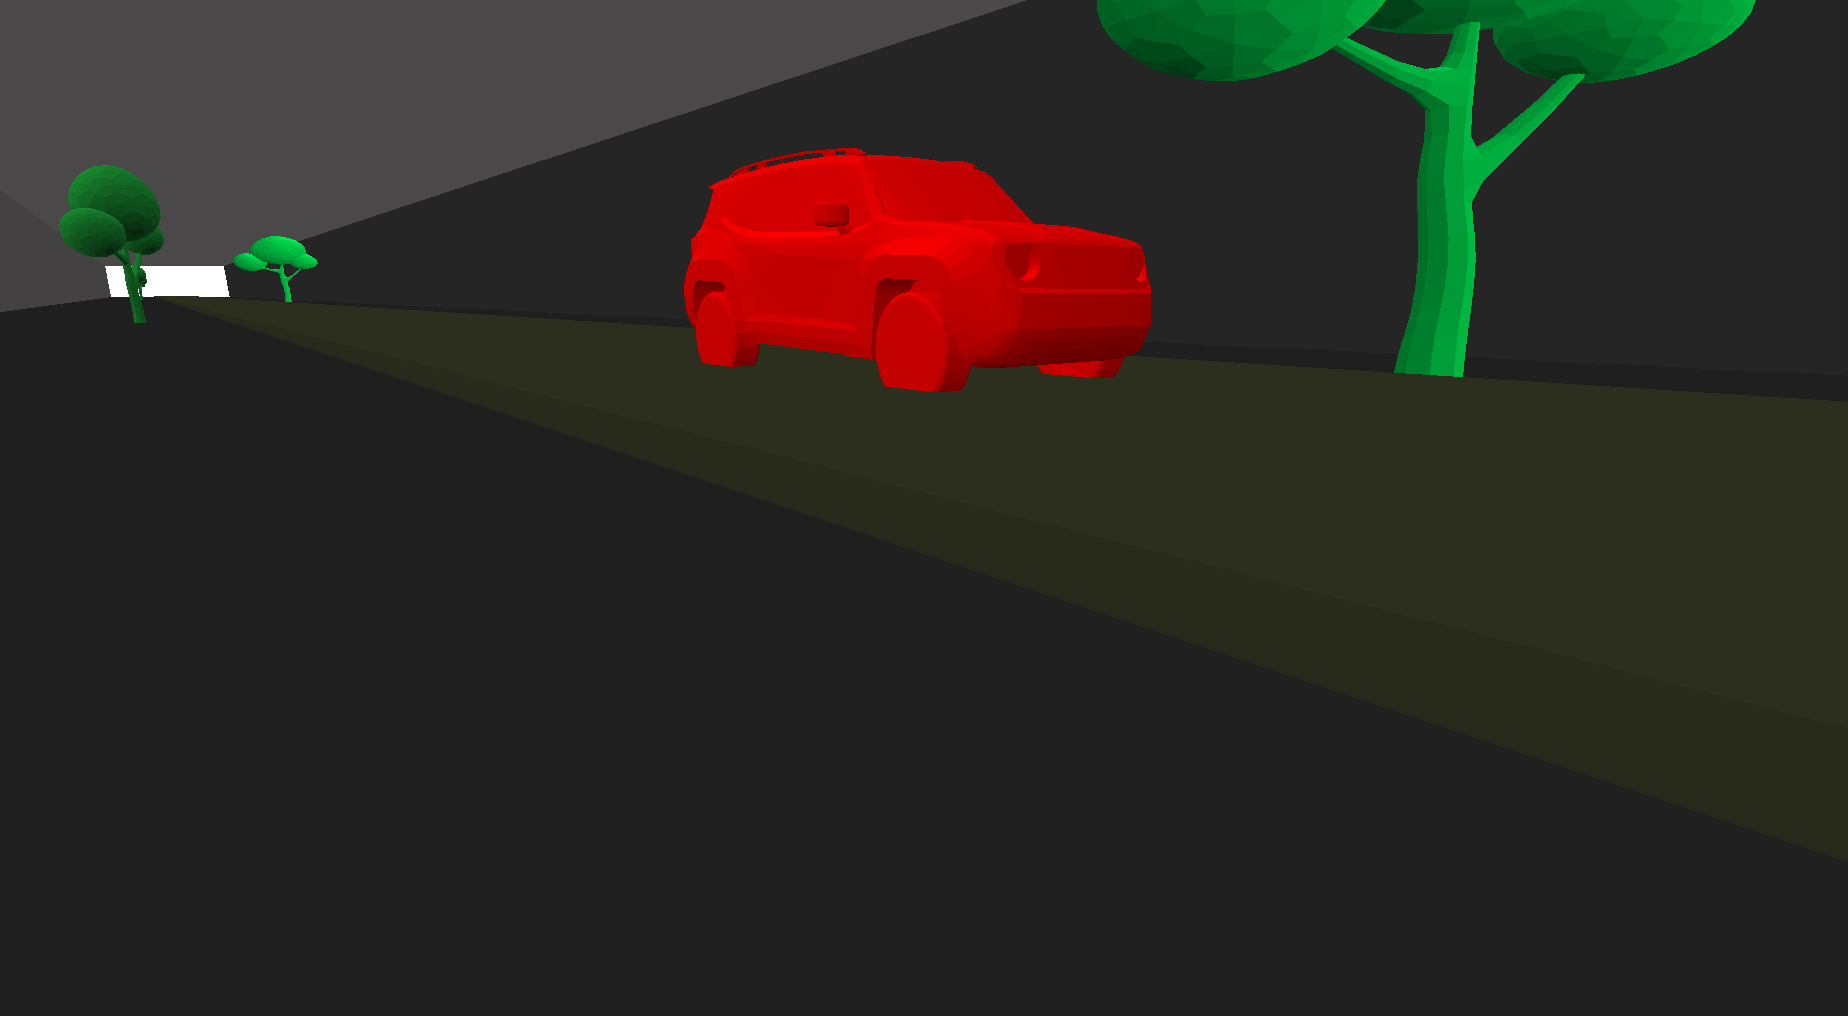
\includegraphics[width=0.8\linewidth]{img/exp/s_1.png} 

    \caption{Сцена, используемая для замеров времени}
    \label{fig:scene_exp}
\end{figure} 


\begin{longtable}{|l|l|}

    \caption{Результаты замеров времени работы этапов построения изображения}
    \label{tbl:time}
    \\
    \hline
        Этап построения                                     & Время, мс \\ \hline    \hline
        буферов кадра, глубины и скорости пикселей          & 14.964   \\ \hline
        буфера максимальной скорости участка                & 0.640    \\ \hline
        размытия с помощью скорости пикселя                 & 1.429    \\ \hline
        размытия с помощью максимальной скорости участка    & 6.204    \\ \hline
\end{longtable}

Из результатов замеров можно сделать вывод, что самым долгим этапом является формирование буферов кадра, глубины и скорости пикселей. Данный этап в 2.2 раза дольше этапов построения размытия с помощью максимальной скорости участка и буфера максимальной скорости участка. И в 10.4 раза больше этапа размытия с помощью скорости пикселя. Из данного факта можно сделать вывод, что методы размытия изображения могут работать в режиме реального времени, но вклад во время формирования итогового изображения зависит от выбранного алгоритма размытия. Данный вопрос будет рассмотрен далее.


\subsection{Анализ времени работы методов размытия от количества семплов}

Было произведено исследование зависимости времени работы методов размытия от количества семплов. Результаты представлены на рисунках \ref{fig:plot_time} и \ref{fig:plot_fps}

\begin{figure}[H]
    \centering
    
    \begin{tikzpicture}
        \begin{axis} [
            legend pos = north west, 
            % ymin = 0, 
            height=0.5\textwidth,
            grid = major,
            xlabel={Количество семплов},
            ylabel={Количество миллисекунд},
            table/col sep = semicolon,
            /pgf/number format/1000 sep={}
        ]
        \legend{ 
            C помощью скорости пикселя,
            C помощью максимальной скорости участка
        };
        \addplot [no markers, thick, blue] table [x=x, y=y] {graphs/samples_pixel.csv};
        \addplot [no markers, thick, red] table [x=x, y=y] {graphs/samples_neighbor.csv};
        % \addplot table [x=x, y=y] {graphs/samples_aprox.csv};
        \end{axis}
    \end{tikzpicture}

    \caption{Зависимость времени генерации итогового изображения для реализаций методов размытия от количества семплов}
    \label{fig:plot_time}
\end{figure} 

\begin{figure}[H]
    \centering
    
    \begin{tikzpicture}
        \begin{axis} [
            legend pos = north east, 
            % ymin = 0, 
            grid = major,
            xlabel={Количество семплов},
            ylabel={Количество кадров в секунду},
            height=0.5\textwidth,
            table/col sep = semicolon,
            /pgf/number format/1000 sep={}
        ]
        \legend{ 
            C помощью скорости пикселя,
            C помощью максимальной скорости участка 
        };
        \addplot [no markers, thick, blue] table [x=x, y=y] {graphs/fps_pixel.csv};
        \addplot [no markers, thick, red] table [x=x, y=y] {graphs/fps_neighbor.csv};
        \end{axis}
    \end{tikzpicture}

    \caption{Зависимость частоты генерации итогового изображения для методов размытия от количества семплов}
    \label{fig:plot_fps}
\end{figure} 

В результате исследования было установлено, что метод размытия с помощью скорости пикселя работает быстрее для исследуемого диапазона количества семплов. Метод размытия с помощью скорости пикселя быстрее метода размытия с помощью максимальной скорости участка и глубины в 1.4 раза при генерации смаза с помощью 40 семплов. Было установлено, что метод размытия с помощью скорости пикселя может работать с частотой обновления кадров 60 Гц при 31 семпле, а метод размытия с помощью максимальной скорости участка и глубины --- при 16 семплах. 

\section{Визуальные характеристики методов размытия}

\subsection{Анализ визуальных характеристик методов размытия от количества семплов}

Были сформированы изображения размытия с помощью скорости участка для разного количества семплов. Они представлены на рисунке \ref{fig:result_samples_neighbor}.

\begin{figure}[h]
    \centering
    \begin{minipage}[h]{0.45\linewidth}
        \center{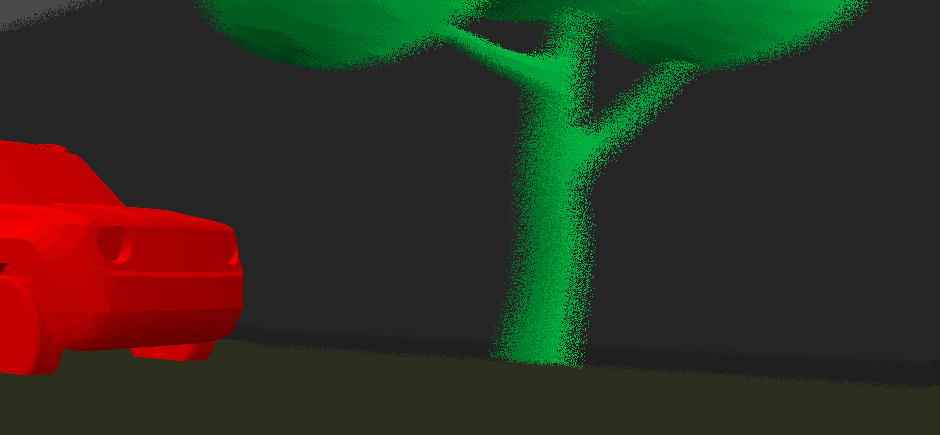
\includegraphics[width=0.99\linewidth]{img/exp/cropped/s_2.png} \\ a)}
    \end{minipage}
    \hfill
    \begin{minipage}[h]{0.45\linewidth}
        \center{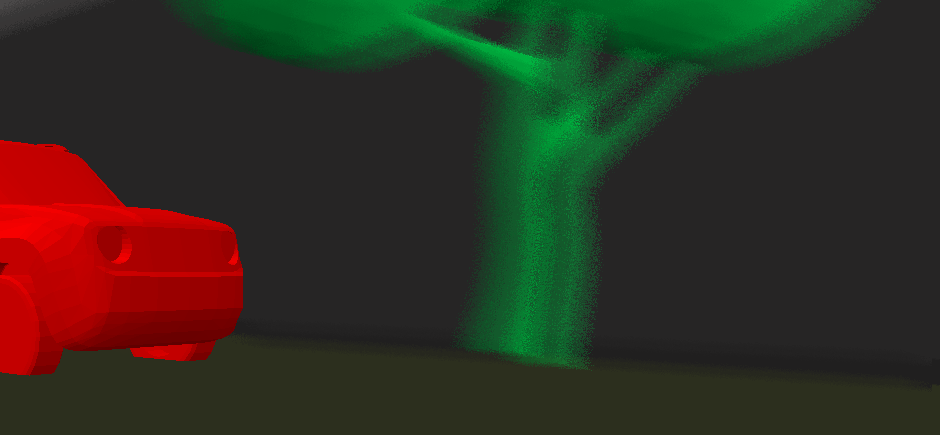
\includegraphics[width=0.99\linewidth]{img/exp/cropped/s_5.png} \\ б)}
    \end{minipage}
    

    \begin{minipage}[h]{0.45\linewidth}
        \center{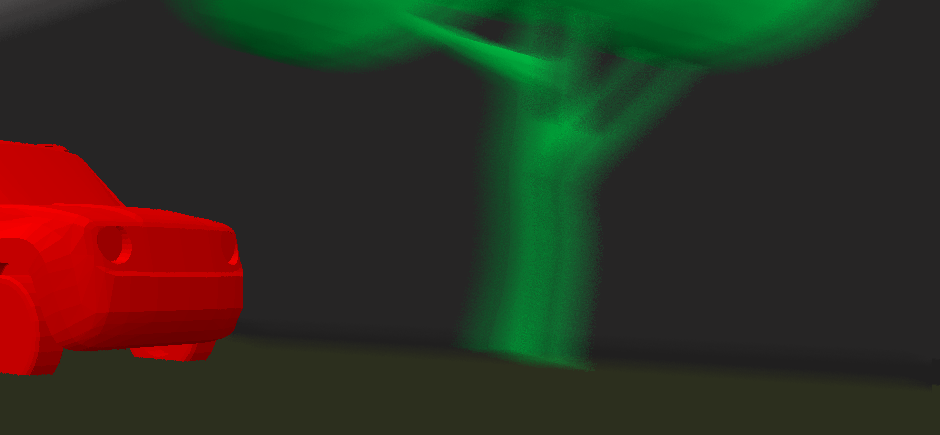
\includegraphics[width=0.99\linewidth]{img/exp/cropped/s_10.png} \\ в)}
    \end{minipage}
    \hfill
    \begin{minipage}[h]{0.45\linewidth}
        \center{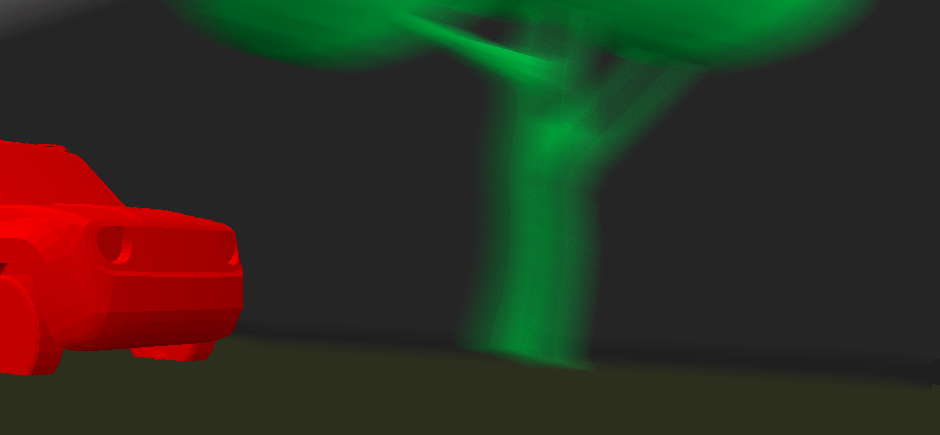
\includegraphics[width=0.99\linewidth]{img/exp/cropped/s_20.png} \\ г)}
    \end{minipage}

    \begin{minipage}[h]{0.45\linewidth}
        \center{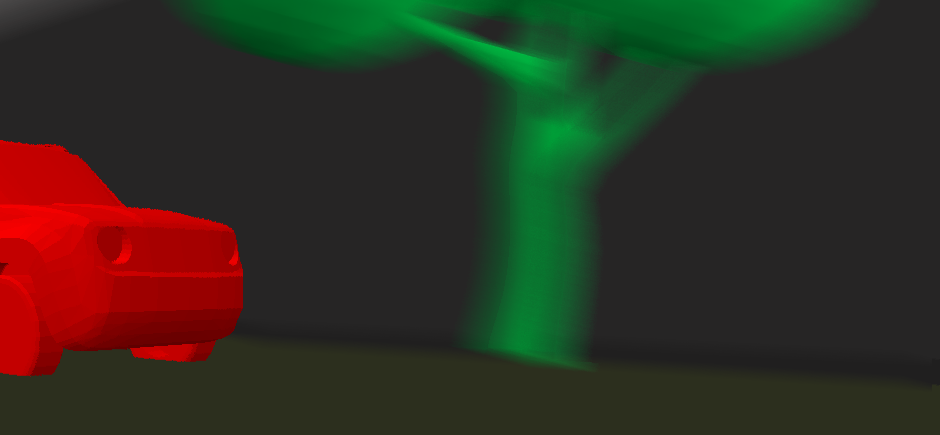
\includegraphics[width=0.99\linewidth]{img/exp/cropped/s_40.png} \\ д)}
    \end{minipage}
    \hfill
    \begin{minipage}[h]{0.45\linewidth}
        \center{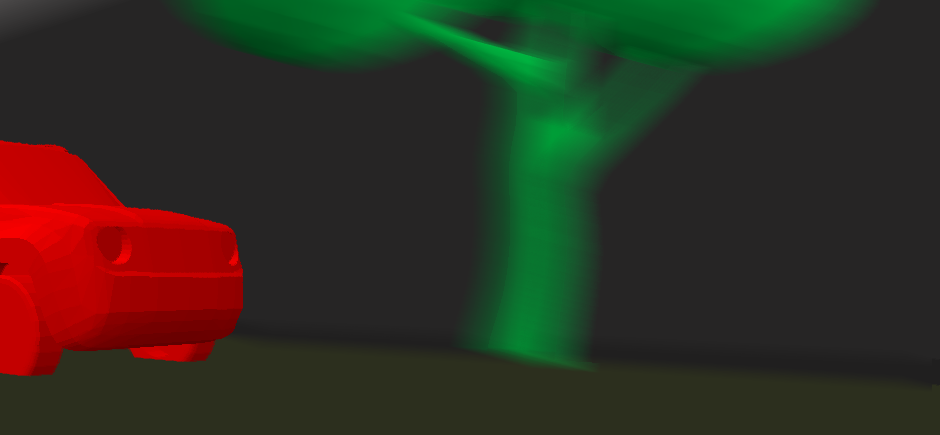
\includegraphics[width=0.99\linewidth]{img/exp/cropped/s_100.png} \\ е)}
    \end{minipage}


    \caption{Результат размытия с помощью скорости участка для \\ а) 2 семплов б) 5 семплов  в) 10 семплов  г) 20 семплов  д) 40 семплов  e) 100 семплов }
    \label{fig:result_samples_neighbor}
\end{figure} 



На изображениях c количеством семплов менее 20 видны недостатки размытия, проявляющиеся в виде шумного смаза. При 20 семплах шум проявляется в меньшей степени. При более 40 семплах результат работы метода не имеет визуальных различий. Из данных утверждений следует, что для изображения среднего качества можно использовать как минимум 20 семплов, а для достижения реалистичности более 40 семплов.

Были сформированы изображения размытия с помощью скорости пикселя для разного количества семплов. Они представлены на рисунке \ref{fig:result_samples_pixel}.


\begin{figure}[H]
    \centering
    \begin{minipage}[h]{0.45\linewidth}
        \center{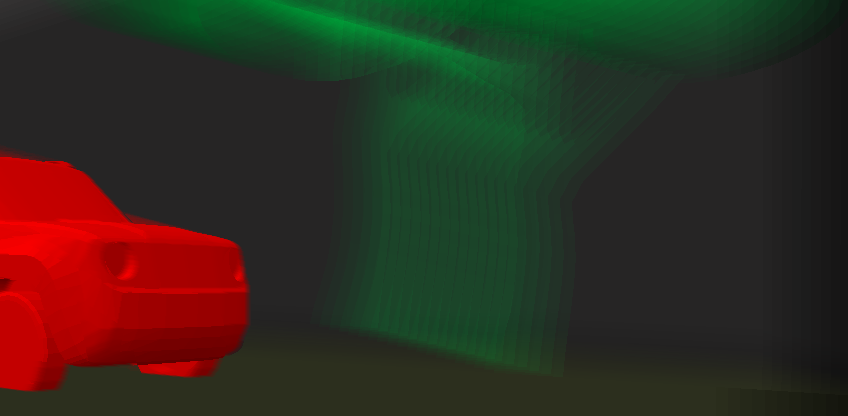
\includegraphics[width=0.99\linewidth]{img/exp/cropped/ss_20.png} \\ a)}
    \end{minipage}
    \hfill
    \begin{minipage}[h]{0.45\linewidth}
        \center{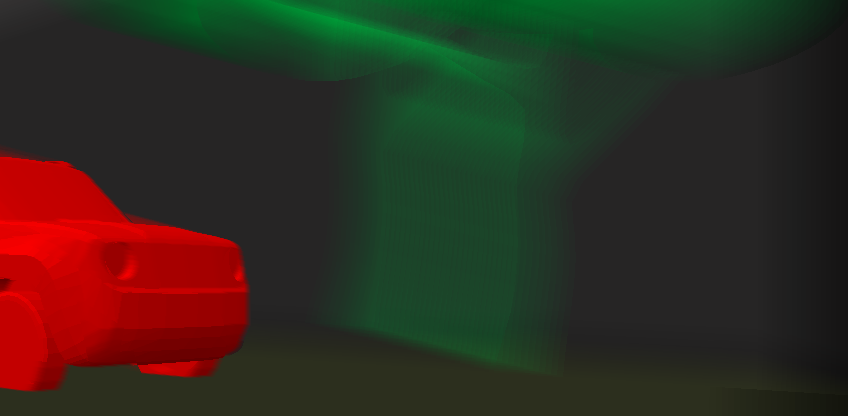
\includegraphics[width=0.99\linewidth]{img/exp/cropped/ss_40.png} \\ б)}
    \end{minipage}

    \begin{minipage}[h]{0.45\linewidth}
        \center{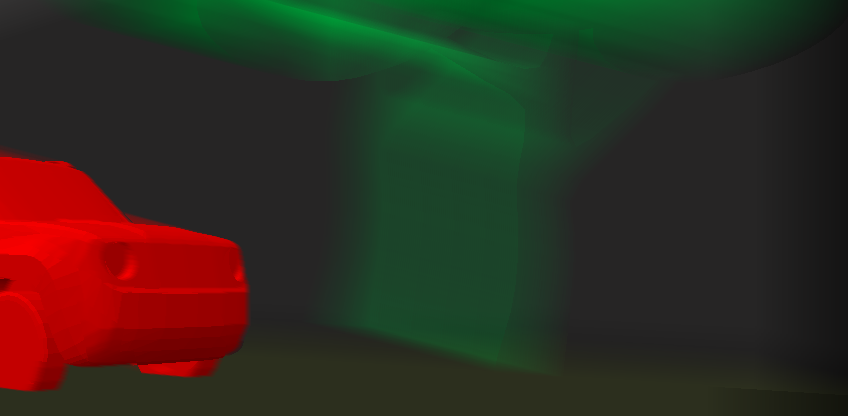
\includegraphics[width=0.99\linewidth]{img/exp/cropped/ss_100.png} \\ в)}
    \end{minipage}
    


    \caption{Результат размытия с помощью скорости пикселя для \\ а) 20 семплов б) 40 семплов  в) 100 семплов}
    \label{fig:result_samples_pixel}
\end{figure} 

На изображениях c количеством семплов менее 40 видны недостатки размытия, проявляющиеся в виде разрывов смаза. При 40 семплах разрывы проявляется в меньшей степени. При более 40 семплах результат работы не имеет разрывов смаза. Из данных утверждений следует, что для изображения среднего качества можно использовать как минимум 40 семплов.


Из данного анализа, можно сделать вывод, что размытие с помощью скорости участка обладает лучшими визуальными характеристиками при равном количестве семплов. Для достижения наилучших визуальных характеристик каждого метода необходимо использовать более 40 семплов.  

\subsection{Анализ визуальных недостатков методов размытия}

В результате исследования были выявлены два визуальных недостатка исследуемых методов размытия. 

Метод размытия с помощью скорости пикселя размывает статичные объекты в системе координат камеры, если задний план находится в движении, а передний статичен.  Метод размытия с помощью скорости участка и буфера глубины лишен данного недостатка в силу учета глубины изображения. Данный визуальный недостаток метода представлен на рисунке \ref{fig:exp_art_1}.


\begin{figure}[H]
    \centering
    \begin{minipage}[h]{0.45\linewidth}
        \center{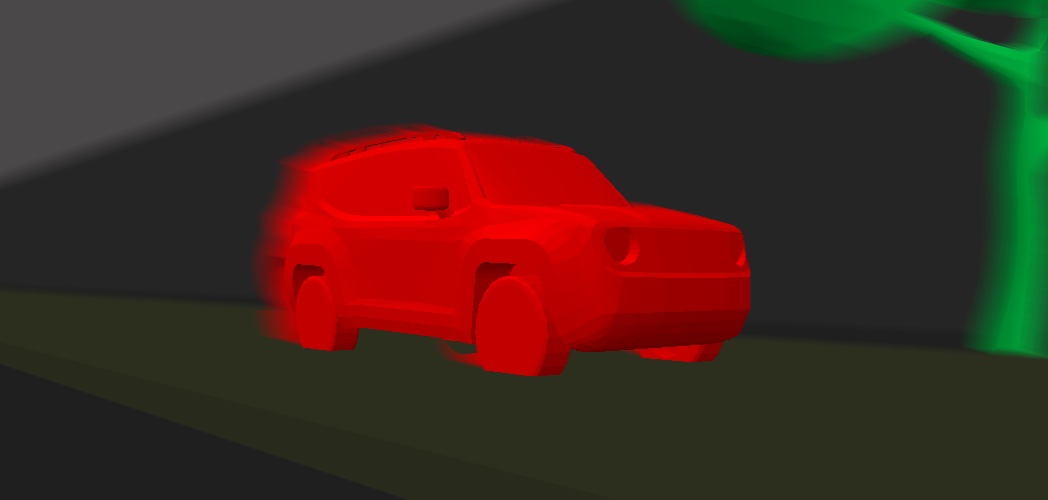
\includegraphics[width=0.99\linewidth]{img/art/cropped/1_pixel.png} \\ a)}
    \end{minipage}
    \hfill
    \begin{minipage}[h]{0.45\linewidth}
        \center{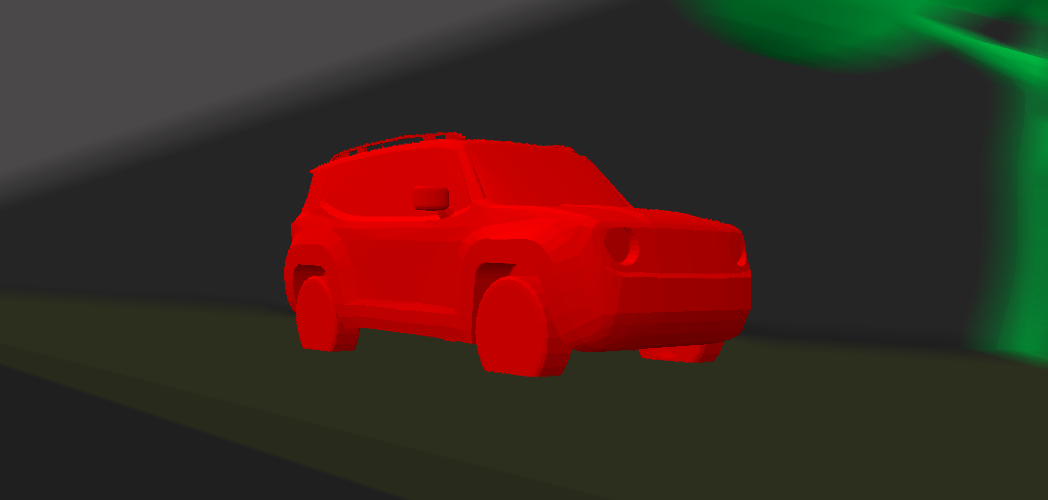
\includegraphics[width=0.99\linewidth]{img/art/cropped/1_neighbor.png} \\ б)}
    \end{minipage}
    

    \caption{Результат размытия с помощью  \\ а) скорости пикселя б) скорости участка и буфера глубины}
    \label{fig:exp_art_1}
\end{figure} 


Другой визуальный недостаток, который был обнаружен, проявляется в потере части смаза из-за перекрытия неподвижным передним планом движущегося объекта и движущегося в том же направлении заднего плана. Данный визуальный недостаток проявляется в двух исследуемых методах. В силу предыдущего визуального недостатка метод размытия с помощью скорости пикселя размывает изображение, используя изображение переднего плана, а метод размытия с помощью скорости участка и буфера глубины не учитывает передний план, но не обладает изображением изображением движущегося объекта из-за чего происходит потеря части смаза. Данный визуальный недостаток методов представлен на рисунке \ref{fig:exp_art_2}.

\begin{figure}[H]
    \centering
    \begin{minipage}[h]{0.45\linewidth}
        \center{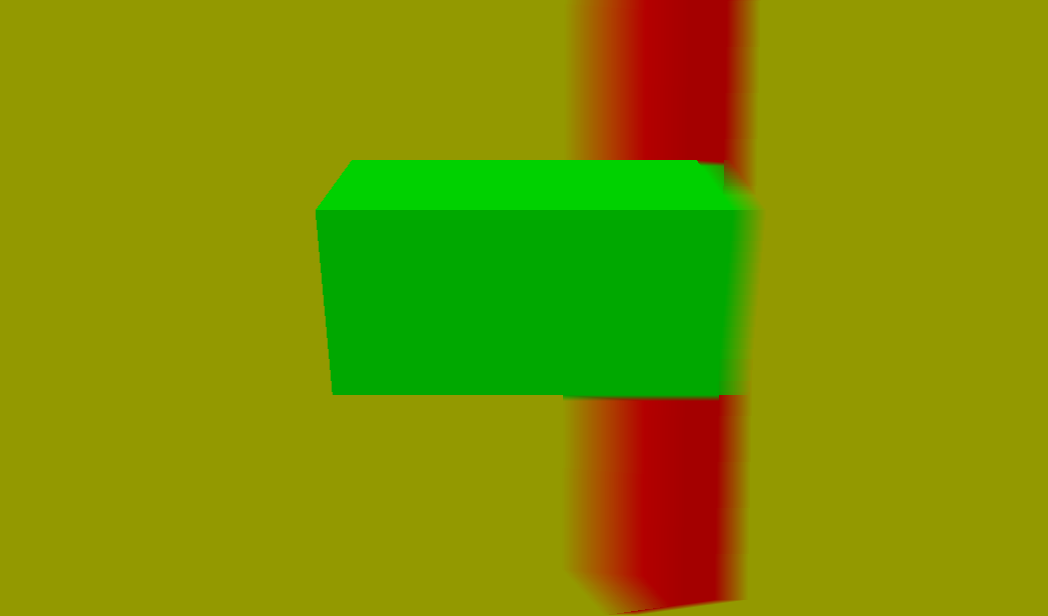
\includegraphics[width=0.99\linewidth]{img/art/cropped/2_pixel.png} \\ a)}
    \end{minipage}
    \hfill
    \begin{minipage}[h]{0.45\linewidth}
        \center{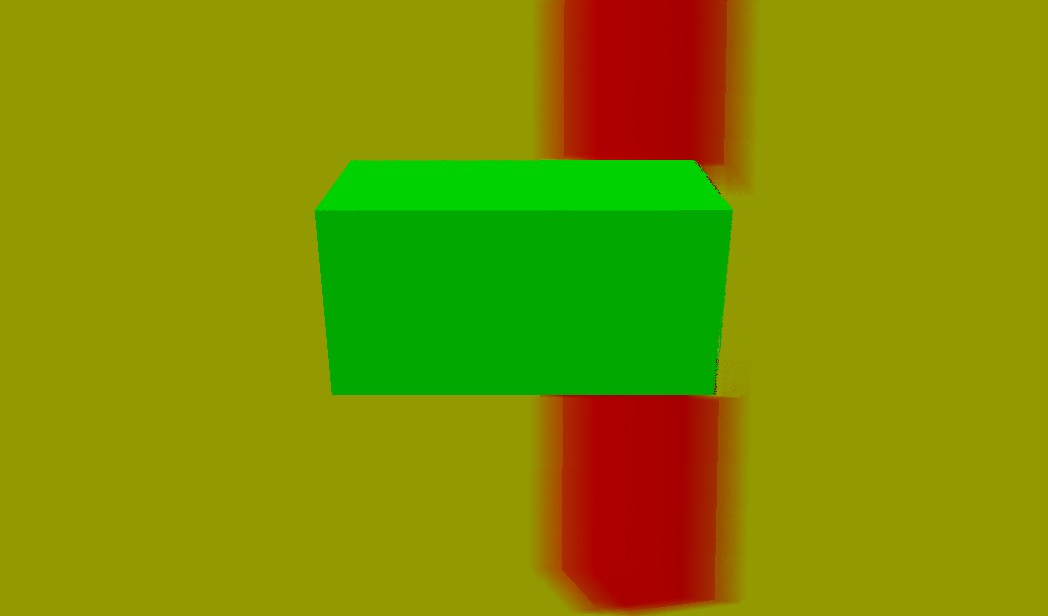
\includegraphics[width=0.99\linewidth]{img/art/cropped/2_neighbor.png} \\ б)}
    \end{minipage}
    

    \caption{Результат размытия с помощью  \\ а) скорости пикселя б) скорости участка и буфера глубины}
    \label{fig:exp_art_2}
\end{figure} 


Необходимо заметить, что данный визуальный недостаток при генерации анимации будет проявляться на малом количестве кадров, что делает его мало заметным при воспроизведении анимации, так как недостаток будет проявляться в течении промежутка времени до 100 мс. Но при генерации одиночных кадров данными методами визуальный недостаток будет проявляться.  


\section{Вывод}


Метод размытия с помощью скорости пикселя может быть использован в режиме реального времени при генерации размытия движения камеры с количеством семплов более 40. При генерации размытия перекрывающихся движущихся объектов могут возникать графические недостатки, которые будут заметны во время воспроизведения анимации. 


Метод размытия с помощью скорости участка и буфера глубины  может быть использован в режиме реального времени при генерации размытия движения камеры и других объектов с количеством семплов не более 40. При этом визуальные недостатки проявляться не будут в течении промежутка времени большего 100 мс.



%%% Local Variables:
%%% mode: latex
%%% TeX-master: "rpz"
%%% End:


% % В данном разделе проводятся вычислительные эксперименты.
% % А на рис.~\ref{fig:spire01} показана схема мыслительного процесса автора...

% % \begin{figure}
% %   \centering
% %   \includegraphics[width=\textwidth]{inc/svg/pic01}
% %   \caption{Как страшно жить}
% %   \label{fig:spire01}
% % \end{figure}


%%% Local Variables:
%%% mode: latex
%%% TeX-master: "rpz"
%%% End:
